% This is samplepaper.tex, a sample chapter demonstrating the
% LLNCS macro package for Springer Computer Science proceedings;
% Version 2.20 of 2017/10/04
%
\documentclass[runningheads]{llncs}
%
\usepackage{amsmath}
\usepackage{booktabs} % For pretty tables
\usepackage{caption} % For caption spacing
\usepackage{subcaption} % For sub-figures
\usepackage{graphicx}
\usepackage{rotating}
\usepackage{pgfplots}
\usepackage[all]{nowidow}
\usepackage[utf8]{inputenc}
\usepackage[margin=1in]{geometry}
\usepackage{tikz}
\usetikzlibrary{er,positioning,bayesnet}
\usepackage{multicol}
\usepackage{algpseudocode,algorithm,algorithmicx}
\usepackage{minted}
\usepackage{hyperref}
\usepackage{siunitx}
\usepackage{esdiff}
\usepackage{float}
\usepackage[inline]{enumitem} % Horizontal lists
% Used for displaying a sample figure. If possible, figure files should
% be included in EPS format.
%
% If you use the hyperref package, please uncomment the following line
% to display URLs in blue roman font according to Springer's eBook style:
% \renewcommand\UrlFont{\color{blue}\rmfamily}

\newcommand{\card}[1]{\left\vert{#1}\right\vert}
\newcommand*\Let[2]{\State #1 $\gets$ #2}
\definecolor{blue}{HTML}{1F77B4}
\definecolor{orange}{HTML}{FF7F0E}
\definecolor{green}{HTML}{2CA02C}

\pgfplotsset{compat=1.14}

\renewcommand{\topfraction}{0.85}
\renewcommand{\bottomfraction}{0.85}
\renewcommand{\textfraction}{0.15}
\renewcommand{\floatpagefraction}{0.8}
\renewcommand{\textfraction}{0.1}
\setlength{\floatsep}{3pt plus 1pt minus 1pt}
\setlength{\textfloatsep}{3pt plus 1pt minus 1pt}
\setlength{\intextsep}{3pt plus 1pt minus 1pt}
\setlength{\abovecaptionskip}{2pt plus 1pt minus 1pt}

\begin{document}

\title{AER303 Aerospace Laboratory - Supersonic Lab}
%\titlerunning{Add subtitle}

\author{Eric Dai\inst{1} \and Jai Willems\inst{2} \and Mingde Yin\inst{3}}
%\authorrunning{F. Author et al.}

\institute{Division of Engineering Science, University of Toronto, Toronto, Canada \email{eric.dai@mail.utoronto.ca}\\ \and Division of Engineering Science, University of Toronto, Toronto, Canada \email{jai.willems@mail.utoronto.ca}\\ \and Division of Engineering Science, University of Toronto, Toronto, Canada\\ \email{mingde.yin@mail.utoronto.ca}}

\maketitle


%%%%%%%%%%%%
% Abstract %
%%%%%%%%%%%%


\begin{abstract}


\keywords{Mach \and Schlieren \and Subsonic \and Supersonic \and Shock Wave}
\end{abstract}


%%%%%%%%%%%%%%%%
% Nomenclature %
%%%%%%%%%%%%%%%%


\newpage
\section{Nomenclature}

Refer to Table \ref{tab:nomenclature} for definitions and symbols common to this report.

\begin{table}[h]
    \centering
    \begin{tabular}{p{4.5cm}p{11cm}}
        \toprule
        Symbol/Term & Description \\
        \midrule
        $A$ & Nozzle cross-sectional area. \\
        $A^*$ & Nozzle cross-sectional area at the throat. \\
        $M$ & Mach number of the flow. \\
        $P$ & Static pressure. \\
        $P_o$ & Total pressure. \\
        $\gamma$ & Ratio of the specific heats of the flow medium. \\
        \bottomrule
    \end{tabular}
    \caption{Commonly used symbols and terms.}
    \label{tab:nomenclature}
\end{table}


%%%%%%%%%%%%%%%%%%%%%%%%%%%%%%%
% Introduction and Background %
%%%%%%%%%%%%%%%%%%%%%%%%%%%%%%%


\newpage
\section{Introduction and Background}\label{sec:introduction_and_background}

This reports aims to explore the pressure and Mach distributions spanning a de Laval nozzle for the subsonic and supersonic mach regimes and compare the theoretically and experimentally attained Mach values. A secondary goal of the report is shock wave visualization using the Schlieren technique. For the remainder of this section, the theoretical introduction to the de Laval nozzle and Mach calculations will be detailed.

\subsection{de Laval Nozzle}

A de Laval nozzle is a special nozzle used to accelerate flow from subsonic to supersonic speeds from the converging-diverging geometry. The de Laval nozzle converges initially to accelerate the flow to reach Mach 1. Subsequent divergence accelerate the flow into the supersonic regime.\newline

\noindent
The area-Mach number relation, seen in equation \ref{eq:background_1}, describes the flow velocity in the de Laval nozzle to its geometry where $A$ is the nozzle cross sectional area, $A^*$ is the nozzle cross sectional area at the throat, $\gamma$ is the ratio of specific heats, and $M$ is the Mach experienced when the flow is passing through a cross section of area $A$.

\begin{equation}
    \frac{A}{A^*}=\frac{1}{M}\left[\frac{2}{\gamma + 1}\left(1 + \frac{\gamma - 1}{2}M^2\right)\right]^{\frac{\gamma + 1}{2(\gamma - 1)}}
    \label{eq:background_1}
\end{equation}

\noindent
Derived from the conservation of mass, the area-Mach number relation captures the behaviour of the de Laval nozzle as seen in figure \ref{fig:AM_relation}. For a subsonic Mach number ($M<1$), a decreasing cross-sectional area corresponds to an increasing Mach number; this is the case for the converging section of the de Laval nozzle. When $A/A^*=1$ (the throat of the nozzle), the Mach number is unity. For supersonic Mach numbers ($M>1$), the Mach number increases with an increasing cross-sectional area; this is characteristic of the de Laval nozzle's diverging section.

\begin{figure}
    \centering
    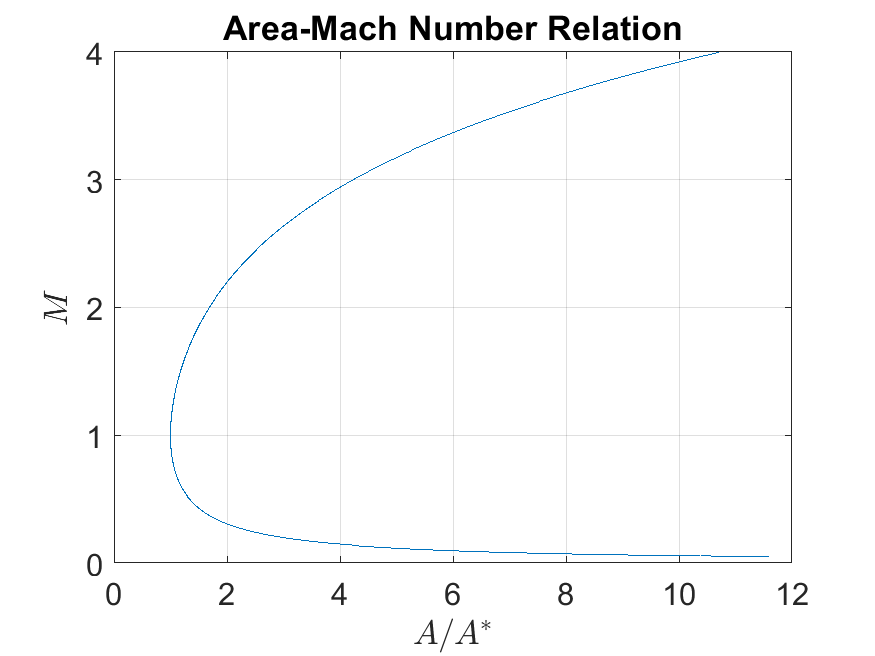
\includegraphics[width=0.7\textwidth]{figures/area_mach_relation.png}
    \caption{Area-Mach number relation for the de Laval nozzle.}
    \label{fig:AM_relation}
\end{figure}

\subsection{Experimental Mach Calculations}

Assuming a one-dimensional and isentropic flow though a de Laval nozzle, the subsonic Mach number can be calculated from experimental pressure data using the isentropic relation given in equation \ref{eq:isentropic_relation}; here, $P_o$ is the total pressure and $P$ is the static pressure. Solving for, the $M$, our isentropic relation takes the form of equation \ref{eq:sub_mach_relation}.

\begin{multicols}{2}
\begin{equation}
    \frac{P_o}{P} = \left(1 + \frac{\gamma - 1}{2}M^2\right)^\frac{\gamma}{\gamma - 1}
    \label{eq:isentropic_relation}
\end{equation}
\begin{equation}
    M^2 = \frac{2}{\gamma - 1}\left[\left(\frac{P_o}{P}\right)^\frac{\gamma - 1}{\gamma} - 1\right]
    \label{eq:sub_mach_relation}
\end{equation}
\end{multicols}

\noindent
In the supersonic case, the static and total pressure measurements are taken on opposite sides of the bow shock formed ahead of the pitot tube. A figment pressure, $P'$, is assumed on the shock, allowing the ratio of the total to static pressure to be as follows:

\begin{align*}
    \frac{P_o}{P} &= \frac{P_o}{P'}\frac{P'}{P} \\
    &= \left(1+\frac{\gamma - 1}{2}M_{<0}^2\right)^{\frac{\gamma}{\gamma - 1}}\left(\frac{2\gamma}{\gamma + 1}M_{>0}^2 - \frac{\gamma - 1}{\gamma + 1}\right)
\end{align*}

\noindent
But the supersonic and subsonic Mach are related using equation \ref{eq:mach_relation}.

\begin{equation}
    M_{<0}^2=\frac{M_{>0}^2+\frac{2}{\gamma - 1}}{\frac{2\gamma}{\gamma - 1}M_{>0}^2 - 1}
    \label{eq:mach_relation}
\end{equation}

\noindent
As a result, the experimental pressure measurements can be directly related to the supersonic Mach using equation \ref{eq:supersonic_mach_relation} which can be numerically solved to get the supersonic Mach value.

\begin{equation}
    \frac{P_o}{P} = \left(\frac{\gamma + 1}{2}M_{>0}^2\right)^{\frac{\gamma}{\gamma - 1}}\left(\frac{2\gamma}{\gamma + 1}M_{>0}^2 - \frac{\gamma - 1}{\gamma + 1}\right)^{-\frac{1}{\gamma - 1}}
    \label{eq:supersonic_mach_relation}
\end{equation}

\subsection{Theoretical Mach Calculations}


%%%%%%%%%%%%%%%%%%%%%%%
% Experimental Set-Up %
%%%%%%%%%%%%%%%%%%%%%%%


\section{Experimental Set-Up}

\noindent
This section details the lab setup and procedure used in the experiment.

\subsection{Apparatus}

\subsection{Procedure}\label{sec:procedure}


%%%%%%%%%%%%%%%%%%%%%%%%%%
% Results and Discussion %
%%%%%%%%%%%%%%%%%%%%%%%%%%


\section{Results and Discussion}


%%%%%%%%%%%%%%%%%%%%
% Sources of Error %
%%%%%%%%%%%%%%%%%%%%


\section{Sources of Error}\label{sec:source_of_error}

\subsection{Quantifiable Sources of Errors}
\begin{table}[H]
\begin{center}
    \begin{tabular}{ll}
        \toprule
        \multicolumn{2}{c}{Quantifiable Error}\\
        \midrule
         & \\
         & \\
        \bottomrule
\end{tabular}
\end{center}
\caption{Quantifiable Sources of Error, Tabulated}
\label{tab:quant_error}
\end{table}


%%%%%%%%%%%%%%
% Conclusion %
%%%%%%%%%%%%%%


\section{Conclusion}


%%%%%%%%%%%%%%%%
% Bibliography %
%%%%%%%%%%%%%%%%


\bibliographystyle{ieeetr}
\bibliography{biblio}


%%%%%%%%%%%%
% Appendix %
%%%%%%%%%%%%


\appendix

\section{Pressure Measurements}

\section{Uncertainty Propagation}

\section{MATLAB and Python Code}

\end{document}